% Chapter 1

\chapter[Introduction]{Introduction} % Main chapter title

\label{Chapter1} % For referencing the chapter elsewhere, use \ref{Chapter1} 

%----------------------------------------------------------------------------------------

% Define some commands to keep the formatting separated from the content 
\newcommand{\keyword}[1]{\textbf{#1}}
\newcommand{\tabhead}[1]{\textbf{#1}}
\newcommand{\code}[1]{\texttt{#1}}
\newcommand{\file}[1]{\texttt{\bfseries#1}}
\newcommand{\option}[1]{\texttt{\itshape#1}}

%----------------------------------------------------------------------------------------

\section{Overview}
Recent years have seen rapid development in robotics technology due the constantly increasing availability of computing power, reductions in the cost of hardware such as digital sensors and actuators, and developments in the application of artificial intelligence to robot control. This has lead to robots being used to perform increasingly complex tasks and solve ever more complex problems. Many new areas of robotics research have emerged as a result, as researchers strive to find new and better ways to apply this technology, entering into problem domains once thought to be impossible for robots. Whole new robotics paradigms have been created as the standard model of a single, very complex, very expensive robot has been questioned, opening the door for cooperative robots, multi-robot systems, and more specifically swarm robotics.

Studies into the self-organising behaviour of social insect colonies, and the development of mathematical models based on these behaviours led to the development of a field of research referred to as Swarm Intelligence (SI). The aim of these models is to determine how large numbers of individual agents are able to solve problems collectively, with each agent using only local information, and without any centralised control. Swarm Robotics developed from a desire to apply these concepts in practice to real world problem solving. Swarm robotics has since emerged as a promising area of research for solving problems which would be infeasibly difficult or expensive for a conventional robotics approach.

%----------------------------------------------------------------------------------------

\section{Project Concept}
Developing and debugging robotics behaviours has always been a challenging task. Whilst traditional software is run in a purely digital environment with a tightly controlled set of inputs and outputs to and from the physical world, robot - by their very nature - must interact constantly with the physical world in order to satisfy their intended purpose. Robots are therefore subject to a much wider array of inputs and outputs, and are subject to a huge number of changing variables within their environment at any given time. This makes detecting, reproducing and correcting faults significantly harder than in traditional software. One of the largest issues is the potential disconnect between the robot's interpretation of the world, the human operators knowledge of this interpretation, and the reality of the world itself. Figure \ref{fig:DebuggingInformation} shows the different layers of information abstraction when dealing with a robotic system. The arrow highlighted in red shows where many of the difficulties in debugging a robot's behaviour occur, as retrieving human readable information from a robot in a timely manner whilst it is running is often non-trivial, and what the robot sees and what the human operator thinks the robot sees may differ significantly.

This problem is compounded significantly when working with multi-robot systems, and especially swarm robotics. Introducing multiple robots multiplies the number potential variables, and the amount of information required to describe the system, increasing both the number of points where a bug may be occurring, and the amount of information the operator needs in order to locate it. The decentralised nature of swarm robotics systems further adds to this problem by not giving the operator any single point where information for the whole system can be retrieved.

This project focuses on mitigating these problems and improving the timeliness with which bugs in a swarm robotics system can be located and fixed by improving the operator's access to system information, collecting that information from multiple sources and presenting it all in one place, in a human readable manner. This project attempts to achieve this by creating a software application and associated wireless data transmission protocols to present a user with a single, coherent, and highly readable interface through which they can view relevant information about the swarm and it's constituent robots in real time. This will be coupled with a video based tracking system to provide the user with a view of the robots' environment augmented with graphical representations of relevant elements of the retrieved data such as sensor readings.

\begin{figure}
\centering
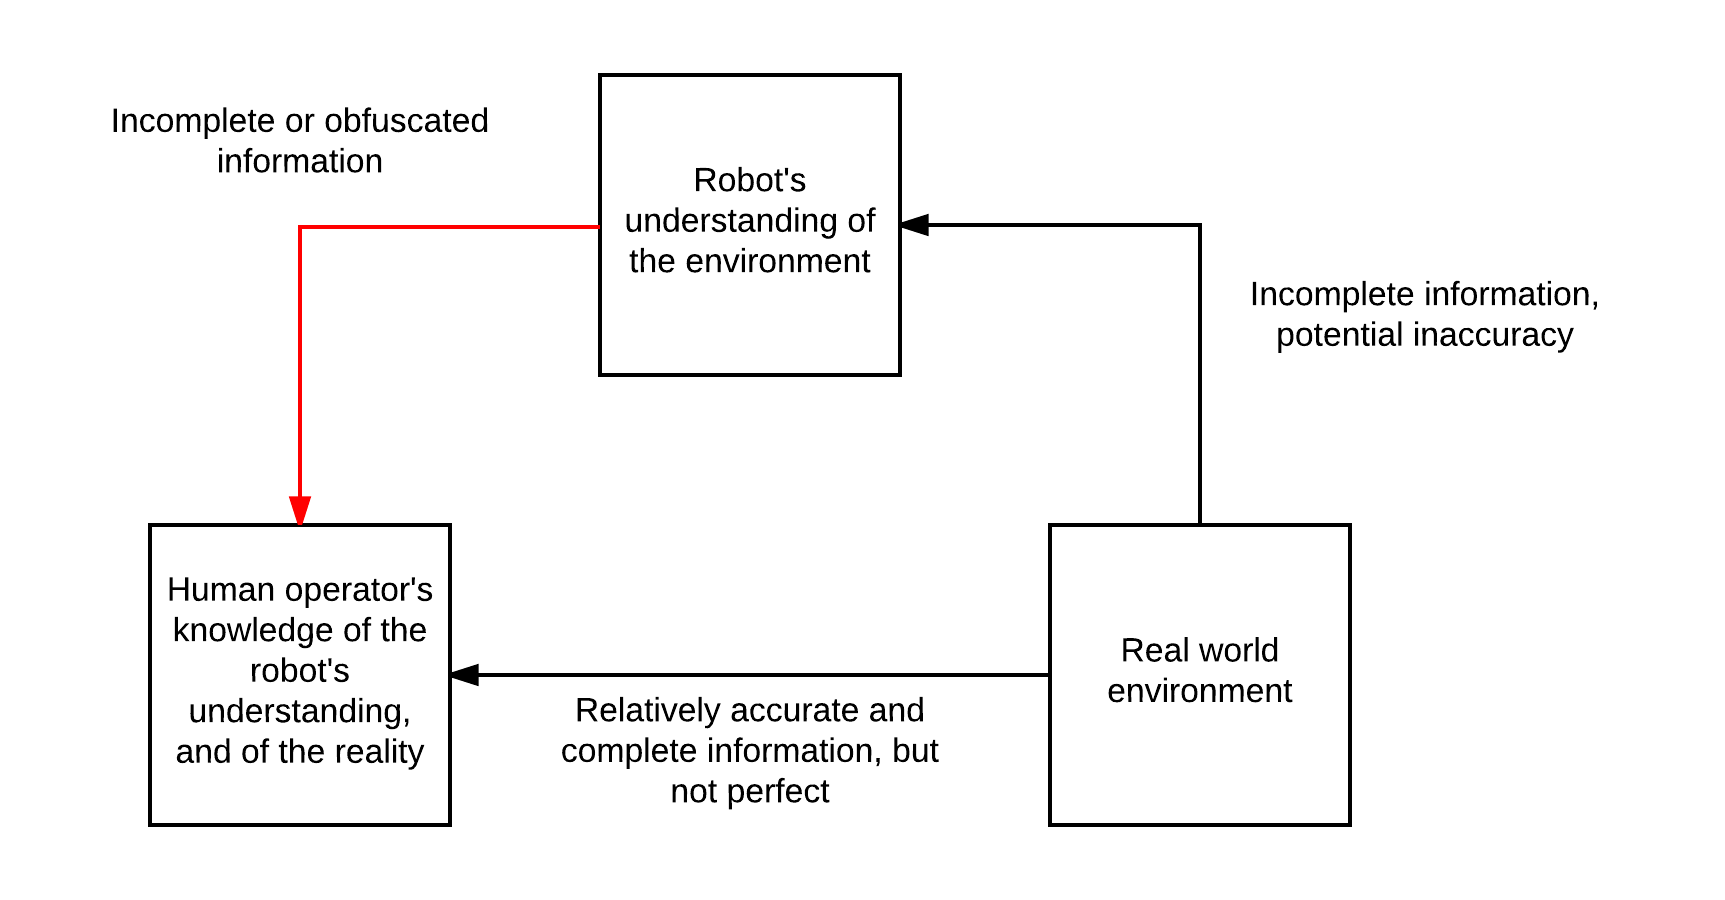
\includegraphics{Figures/RobotDebuggingInformationAbstraction.png}
\decoRule
\caption[Debugging Information]{Layers of information abstraction in robotics debugging.}
\label{fig:DebuggingInformation}
\end{figure}
